% Options for packages loaded elsewhere
\PassOptionsToPackage{unicode}{hyperref}
\PassOptionsToPackage{hyphens}{url}
%
\documentclass[
]{article}
\usepackage{lmodern}
\usepackage{amssymb,amsmath}
\usepackage{ifxetex,ifluatex}
\ifnum 0\ifxetex 1\fi\ifluatex 1\fi=0 % if pdftex
  \usepackage[T1]{fontenc}
  \usepackage[utf8]{inputenc}
  \usepackage{textcomp} % provide euro and other symbols
\else % if luatex or xetex
  \usepackage{unicode-math}
  \defaultfontfeatures{Scale=MatchLowercase}
  \defaultfontfeatures[\rmfamily]{Ligatures=TeX,Scale=1}
\fi
% Use upquote if available, for straight quotes in verbatim environments
\IfFileExists{upquote.sty}{\usepackage{upquote}}{}
\IfFileExists{microtype.sty}{% use microtype if available
  \usepackage[]{microtype}
  \UseMicrotypeSet[protrusion]{basicmath} % disable protrusion for tt fonts
}{}
\makeatletter
\@ifundefined{KOMAClassName}{% if non-KOMA class
  \IfFileExists{parskip.sty}{%
    \usepackage{parskip}
  }{% else
    \setlength{\parindent}{0pt}
    \setlength{\parskip}{6pt plus 2pt minus 1pt}}
}{% if KOMA class
  \KOMAoptions{parskip=half}}
\makeatother
\usepackage{xcolor}
\IfFileExists{xurl.sty}{\usepackage{xurl}}{} % add URL line breaks if available
\IfFileExists{bookmark.sty}{\usepackage{bookmark}}{\usepackage{hyperref}}
\hypersetup{
  pdftitle={Landmarking Protocol 3d2 for gahaganmorph3},
  pdfauthor={Robert Z. Selden, Jr.},
  hidelinks,
  pdfcreator={LaTeX via pandoc}}
\urlstyle{same} % disable monospaced font for URLs
\usepackage[margin=1in]{geometry}
\usepackage{color}
\usepackage{fancyvrb}
\newcommand{\VerbBar}{|}
\newcommand{\VERB}{\Verb[commandchars=\\\{\}]}
\DefineVerbatimEnvironment{Highlighting}{Verbatim}{commandchars=\\\{\}}
% Add ',fontsize=\small' for more characters per line
\usepackage{framed}
\definecolor{shadecolor}{RGB}{248,248,248}
\newenvironment{Shaded}{\begin{snugshade}}{\end{snugshade}}
\newcommand{\AlertTok}[1]{\textcolor[rgb]{0.94,0.16,0.16}{#1}}
\newcommand{\AnnotationTok}[1]{\textcolor[rgb]{0.56,0.35,0.01}{\textbf{\textit{#1}}}}
\newcommand{\AttributeTok}[1]{\textcolor[rgb]{0.77,0.63,0.00}{#1}}
\newcommand{\BaseNTok}[1]{\textcolor[rgb]{0.00,0.00,0.81}{#1}}
\newcommand{\BuiltInTok}[1]{#1}
\newcommand{\CharTok}[1]{\textcolor[rgb]{0.31,0.60,0.02}{#1}}
\newcommand{\CommentTok}[1]{\textcolor[rgb]{0.56,0.35,0.01}{\textit{#1}}}
\newcommand{\CommentVarTok}[1]{\textcolor[rgb]{0.56,0.35,0.01}{\textbf{\textit{#1}}}}
\newcommand{\ConstantTok}[1]{\textcolor[rgb]{0.00,0.00,0.00}{#1}}
\newcommand{\ControlFlowTok}[1]{\textcolor[rgb]{0.13,0.29,0.53}{\textbf{#1}}}
\newcommand{\DataTypeTok}[1]{\textcolor[rgb]{0.13,0.29,0.53}{#1}}
\newcommand{\DecValTok}[1]{\textcolor[rgb]{0.00,0.00,0.81}{#1}}
\newcommand{\DocumentationTok}[1]{\textcolor[rgb]{0.56,0.35,0.01}{\textbf{\textit{#1}}}}
\newcommand{\ErrorTok}[1]{\textcolor[rgb]{0.64,0.00,0.00}{\textbf{#1}}}
\newcommand{\ExtensionTok}[1]{#1}
\newcommand{\FloatTok}[1]{\textcolor[rgb]{0.00,0.00,0.81}{#1}}
\newcommand{\FunctionTok}[1]{\textcolor[rgb]{0.00,0.00,0.00}{#1}}
\newcommand{\ImportTok}[1]{#1}
\newcommand{\InformationTok}[1]{\textcolor[rgb]{0.56,0.35,0.01}{\textbf{\textit{#1}}}}
\newcommand{\KeywordTok}[1]{\textcolor[rgb]{0.13,0.29,0.53}{\textbf{#1}}}
\newcommand{\NormalTok}[1]{#1}
\newcommand{\OperatorTok}[1]{\textcolor[rgb]{0.81,0.36,0.00}{\textbf{#1}}}
\newcommand{\OtherTok}[1]{\textcolor[rgb]{0.56,0.35,0.01}{#1}}
\newcommand{\PreprocessorTok}[1]{\textcolor[rgb]{0.56,0.35,0.01}{\textit{#1}}}
\newcommand{\RegionMarkerTok}[1]{#1}
\newcommand{\SpecialCharTok}[1]{\textcolor[rgb]{0.00,0.00,0.00}{#1}}
\newcommand{\SpecialStringTok}[1]{\textcolor[rgb]{0.31,0.60,0.02}{#1}}
\newcommand{\StringTok}[1]{\textcolor[rgb]{0.31,0.60,0.02}{#1}}
\newcommand{\VariableTok}[1]{\textcolor[rgb]{0.00,0.00,0.00}{#1}}
\newcommand{\VerbatimStringTok}[1]{\textcolor[rgb]{0.31,0.60,0.02}{#1}}
\newcommand{\WarningTok}[1]{\textcolor[rgb]{0.56,0.35,0.01}{\textbf{\textit{#1}}}}
\usepackage{graphicx,grffile}
\makeatletter
\def\maxwidth{\ifdim\Gin@nat@width>\linewidth\linewidth\else\Gin@nat@width\fi}
\def\maxheight{\ifdim\Gin@nat@height>\textheight\textheight\else\Gin@nat@height\fi}
\makeatother
% Scale images if necessary, so that they will not overflow the page
% margins by default, and it is still possible to overwrite the defaults
% using explicit options in \includegraphics[width, height, ...]{}
\setkeys{Gin}{width=\maxwidth,height=\maxheight,keepaspectratio}
% Set default figure placement to htbp
\makeatletter
\def\fps@figure{htbp}
\makeatother
\setlength{\emergencystretch}{3em} % prevent overfull lines
\providecommand{\tightlist}{%
  \setlength{\itemsep}{0pt}\setlength{\parskip}{0pt}}
\setcounter{secnumdepth}{-\maxdimen} % remove section numbering

\title{Landmarking Protocol 3d2 for gahaganmorph3}
\author{Robert Z. Selden, Jr.}
\date{11/13/2020}

\begin{document}
\maketitle

The landmarking protocol (LM3d2) developed for this project represents a
substantial methodological advancement when contrasted with those
protocols used in previous studies of Gahagan biface morphology (Selden
Jr., Dockall, and Shafer 2018; Selden Jr., Dockall, and Dubied 2020).
This protocol represents the continued evolution of a research programme
concerned with the development of a rigorous and replicable
three-dimensional (3D) landmarking workflow, which simultaneously takes
into account the unique and complex design elements associated with
individual bifaces. Landmark (LM) and semilandmark (sLM) placement was
achieved through the construction of reference geometry in
\emph{Geomagic Design X (Build Version 2020.0.2 {[}Build Number:
55{]})}, used to expand upon the previous LM configuration, and
capitalise upon additional design attributes. Reference geometry
provides the requisite foundation needed to apply the LM and sLM points
at mathematically-defined locations. The result is a LM and sLM
configuration that articulates with specific morphological features
(plan views, profiles, and cross-sections), which have demonstrated
utility in wide-ranging studies of biface and projectile point
morphology.

\hypertarget{foundations}{%
\subsection{Foundations}\label{foundations}}

The initial landmarking protocol enlisted a curve that was projected
onto a 2D plane. That protocol provided the framework needed to begin a
more thorough consideration of 3D landmarking protocols, driving the
evolution of the landmarking protocol described here.

\begin{Shaded}
\begin{Highlighting}[]
\NormalTok{knitr}\OperatorTok{::}\KeywordTok{include_graphics}\NormalTok{(}\StringTok{'images/gahaganmorph.jpg'}\NormalTok{)}
\end{Highlighting}
\end{Shaded}

\begin{figure}
\includegraphics[width=47.76in]{images/gahaganmorph} \caption{The landmarking protocol used in the 2D analysis of Gahagan bifaces, where all landmarks and semilandmarks were projected onto a plane.}\label{fig:fig.gahaganmorph}
\end{figure}

The first 3D landmarking protocol
(\href{https://github.com/aksel-blaise/gahaganmorph2/blob/master/analysis/landmarking-protocol.md}{LM3d1})
used for an analysis of Gahagan bifaces focused only upon the plan view
(lateral/basal edges), and enlisted \emph{auto3dgm} to achieve the
principal alignments needed to assign the front and back to each face.
While basic, this landmarking protocol generated the requisite framework
needed to begin constructing different suites of design-driven
\texttt{reference\ geometry} that can be tailored to address specific
research questions.

\begin{Shaded}
\begin{Highlighting}[]
\NormalTok{knitr}\OperatorTok{::}\KeywordTok{include_graphics}\NormalTok{(}\StringTok{'images/gahaganmorph2.png'}\NormalTok{)}
\end{Highlighting}
\end{Shaded}

\begin{figure}
\includegraphics[width=53.12in]{images/gahaganmorph2} \caption{The first [3D landmarking protocol](https://github.com/aksel-blaise/gahaganmorph2/blob/master/analysis/landmarking-protocol.md) (LM3d1) used to analyse Gahagan bifaces, which captured those attributes associated with axial twisting.}\label{fig:fig.gahaganmorph2}
\end{figure}

The goal of this effort was to increase the precision and rigor of the
study by including additional elements from the Z-dimension to capture
those morphological characteristics associated with plan, profile, and
cross-sections. This landmarking protocol is the culmination of the
iterative design process that began during the previous 2D (Selden Jr.,
Dockall, and Shafer 2018) and 3D
(\href{https://github.com/aksel-blaise/gahaganmorph2/blob/master/analysis/landmarking-protocol.md}{LM3d1})
(Selden Jr., Dockall, and Dubied 2020) geometric morphometric analyses.
The cross-sections increase the coverage of sLMs across mesh topology,
providing for greater precision in the analysis of whole-object
morphology, and can be subset as a means of analyzing specific features
of interest. For this study, the previously-noted morphological
differences that occur in plan view (Selden Jr., Dockall, and Shafer
2018; Selden Jr., Dockall, and Dubied 2020) are further scrutinized in
an effort to explore whether those differences in Gahagan biface plan
view might be said to extend to the profiles of Gahagan bifaces. Due to
the degree of axial twisting that occurs across the sample, it is not
possible to gather the data needed to answer this query using 2D
methods.

The continued evolution of this landmarking protocol represents a
concerted effort to better comprehend the vagaries of morphological
similarities and differences among Gahagan bifaces. While true that some
landmarking protocols can be---and often are---recycled as new specimens
are added, this research program endeavors to achieve ever-greater
accuracy and precision in each subsequent iteration.

\hypertarget{generating-the-peripheral-plan-view-spline}{%
\subsection{Generating the peripheral (plan view)
spline}\label{generating-the-peripheral-plan-view-spline}}

This effort begins with a spline extracted from the surface geometry of
the mesh using the \texttt{extract\ contour\ curves} command. In
reverse-engineering, \texttt{extract\ contour\ curves} is regularly
employed as the first step in building a \texttt{patch\ network} to
construct a surface. The extracted feature curve is rendered as a
spline, and follows the highest curvature contours around the periphery
of the lateral and basal edges, following the highly variable sinuous
edge morphology around the entirety of each biface (Selden Jr., Dockall,
and Dubied 2020). The remainder of the landmarking protocol is based
upon this spline, which was subsequently split at four
mathematically-defined locations (Selden Jr., Dockall, and Dubied 2020).

\begin{Shaded}
\begin{Highlighting}[]
\NormalTok{knitr}\OperatorTok{::}\KeywordTok{include_graphics}\NormalTok{(}\StringTok{'images/extractspline.png'}\NormalTok{)}
\end{Highlighting}
\end{Shaded}

\begin{figure}
\includegraphics[width=1\linewidth]{images/extractspline} \caption{Spline extracted along the highest contours of the projectile.}\label{fig:figspline}
\end{figure}

\hypertarget{splitting-spline-1}{%
\subsubsection{Splitting Spline 1}\label{splitting-spline-1}}

\emph{\texttt{Reference\ geometries} are used in the assistance of
creating other features. These include basic geometric entities, such as
\texttt{planes}, \texttt{vectors}, \texttt{coordinates},
\texttt{points}, and \texttt{polygons}. A \texttt{reference\ point} is a
virtual point and is used to mark a specific position on a model or in
3D space. A \texttt{reference\ plane} is a virtual plane that has a
normal direction and an infinite size. A \texttt{reference\ plane} is
not a surface body, and is used to create other features.}

The characteristic points and tangents developed for this landmarking
protocol were inspired by the work of Birkhoff (1933), which has been
gainfully employed within the context of both ceramic (Selden Jr. 2018a,
2018b, 2019, 2021) and lithic analyses (Selden Jr., Dockall, and Shafer
2018; Selden Jr., Dockall, and Dubied 2020).

\hypertarget{split-spline-1-at-location-of-lm-01}{%
\paragraph{Split Spline 1 at location of LM
01}\label{split-spline-1-at-location-of-lm-01}}

The \texttt{horizontal\ tangent} was calculated by drawing a horizontal
line above the tip of each biface using the tangent as a
\texttt{common\ constraint}, and the \texttt{horizontal} as the
\texttt{independent\ constraint}. To split the 3D spline at the location
of the \texttt{horizontal\ tangent}, a \texttt{reference\ point} was
inserted at the location of the \texttt{tangent} in the 2D sketch (light
blue point; below, left), followed by a \texttt{reference\ plane} (in
white; below, left and right) using the
\texttt{pick\ point\ and\ normal\ axis} function where the
\texttt{reference\ point} (h-tangent) was used as the
\texttt{pick\ point}, and the \texttt{Right\ plane} as the
\texttt{normal\ axis} (below, left). The 3D spline was cut at the
location where the \texttt{reference\ plane} intersected with the spline
(below image, right).

\begin{Shaded}
\begin{Highlighting}[]
\NormalTok{knitr}\OperatorTok{::}\KeywordTok{include_graphics}\NormalTok{(}\StringTok{'images/lm1.png'}\NormalTok{)}
\end{Highlighting}
\end{Shaded}

\begin{figure}
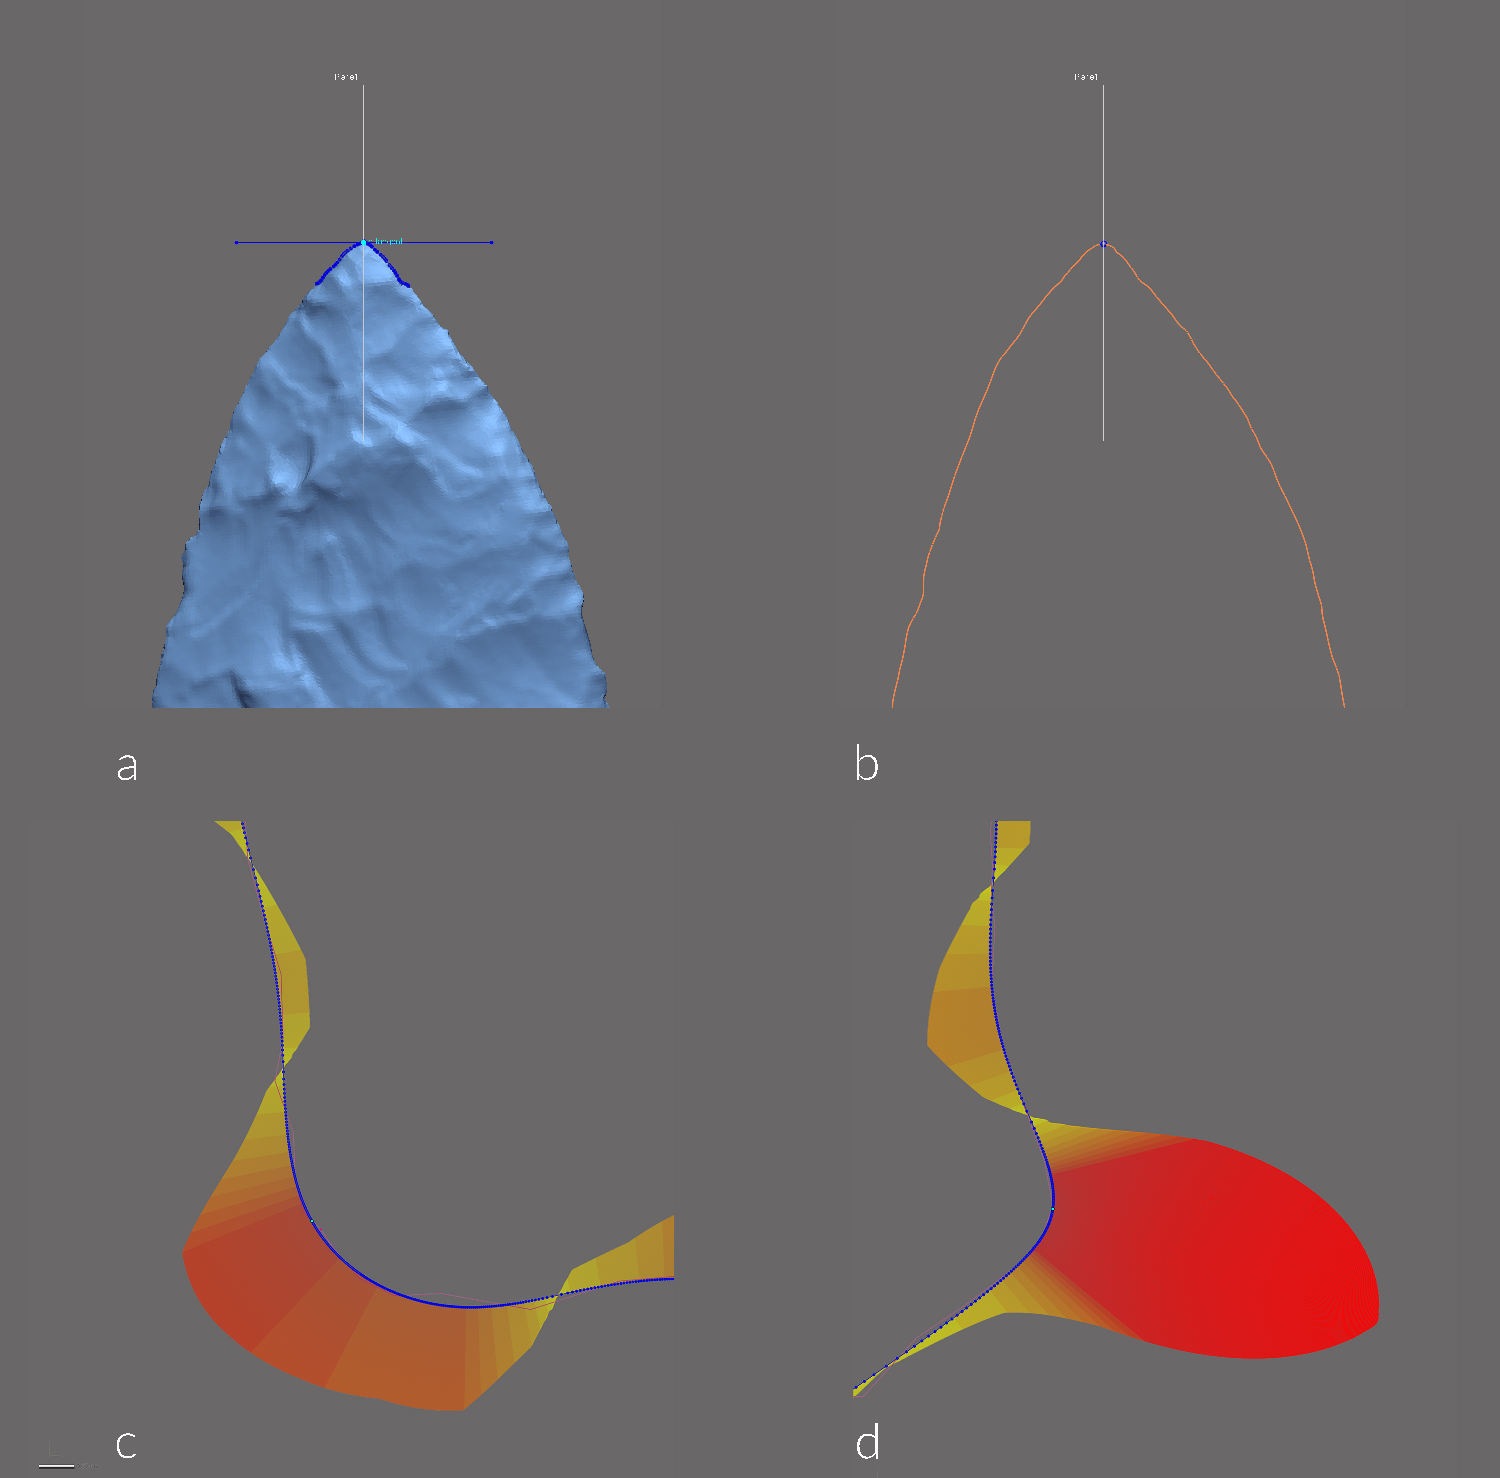
\includegraphics[width=1\linewidth]{images/lm1} \caption{Identify horizontal tangent, insert reference point and reference plane (left). Use reference plane to cut spline at the location of the horizontal tangent (right).}\label{fig:figlm1}
\end{figure}

\hypertarget{split-spline-1-at-locations-of-lm-02-and-lm-03}{%
\paragraph{Split Spline 1 at locations of LM 02 and LM
03}\label{split-spline-1-at-locations-of-lm-02-and-lm-03}}

The point of highest curvature on either side of the basal edge was
calculated using the \texttt{curvature} function in the Accuracy
Analyzer. This function displays the curvature flow as a continuous
color plot across the area of the curve. In this instance,
\emph{curvature} is defined as the amount by which a geometric shape
deviates from being flat or straight in the case of a line. Curvature is
displayed in different colors according to the local radius, and
calculated in only one direction (U or V) along the curve. Using this
tool, the two points of highest curvature were located between the basal
and lateral edges on either side of each projectile where the local
radius measure was largest. The orientation of each biface was initially
dictated by the \emph{auto3dgm} alignment in
\href{https://github.com/aksel-blaise/gahaganmorph2/blob/master/analysis/landmarking-protocol.md}{LM3d1};
however, \emph{LM3d2 follows a different protocol.}

\begin{Shaded}
\begin{Highlighting}[]
\NormalTok{knitr}\OperatorTok{::}\KeywordTok{include_graphics}\NormalTok{(}\StringTok{'images/splinesplit1.png'}\NormalTok{)}
\end{Highlighting}
\end{Shaded}

\begin{figure}
\includegraphics[width=1\linewidth]{images/splinesplit1} \caption{Identify points of hightest curvature (light blue) at left/right intersection of lateral and basal edges.}\label{fig:figcurve}
\end{figure}

\hypertarget{split-spline-1-at-location-of-lm-04}{%
\paragraph{Split Spline 1 at location of LM
04}\label{split-spline-1-at-location-of-lm-04}}

One additional landmark (LM 06) was placed at the center of the base.
The location of this landmark was identified by calculating the linear
distance between LM 02 and LM 03, and projecting a
\texttt{reference\ point} (ctrl-div; below) equidistant between the two.
A \texttt{reference\ plane} was added using the ctrl-div as the pick
point, and the \texttt{Right\ plane} as the \texttt{normal\ axis}. The
spline was then split at the intersection of the
\texttt{reference\ plane} and the basal spline.

\begin{Shaded}
\begin{Highlighting}[]
\NormalTok{knitr}\OperatorTok{::}\KeywordTok{include_graphics}\NormalTok{(}\StringTok{'images/lm4.png'}\NormalTok{)}
\end{Highlighting}
\end{Shaded}

\begin{figure}
\includegraphics[width=1\linewidth]{images/lm4} \caption{Calculate linear distance between LM2 and LM3, insert reference plane coplanar to Right plane equidistant between LM2 and LM3, and use the reference plane to cut the spline.}\label{fig:figlm4}
\end{figure}

\hypertarget{reference-geometry-build-1}{%
\subsection{Reference geometry, Build
1}\label{reference-geometry-build-1}}

Each of the preceding protocols were used in the previous analysis of
Gahagan bifaces (Selden Jr., Dockall, and Dubied 2020), and the
following sections detail the logical evolution of that landmarking
protocol. The resulting constellation of LM and sLM points can be subset
to test a wide range of hypotheses associated with the plan and profile
views of bifaces, and can be extended to include specific or multiple
components of each cross-section. Each cross-section is also split
between LM 01 and LM04, allowing for analyses of \emph{bilateral
asymmetry} for both plan and profile views.

\hypertarget{reference-vector-1-point-2-and-plane-2}{%
\subsubsection{Reference Vector 1, Point 2, and Plane
2}\label{reference-vector-1-point-2-and-plane-2}}

A linear \texttt{reference\ vector} (vector.1) was inserted between LM
01 and LM 04, and a \texttt{reference\ point} (ref.pt.2) was placed
equidistant between LMs 02 and 03 along vector.1. The Z-coordinates of
ref.pt.2 were altered to relocate it 15mm from vector.1 in the direction
of the Z-axis, while otherwise maintaining its' alignment with vector 1.
The \texttt{pick\ point\ and\ coplanar} function was used to place a
\texttt{reference\ plane} (ref.pl.2) along vector.1 in the direction of
ref.pt.2, bisecting the biface along the Z-axis---perpendicular to the
lateral edges---between LM 01 and LM 04.

\begin{Shaded}
\begin{Highlighting}[]
\NormalTok{knitr}\OperatorTok{::}\KeywordTok{include_graphics}\NormalTok{(}\StringTok{'images/vecptplane.png'}\NormalTok{)}
\end{Highlighting}
\end{Shaded}

\begin{figure}
\includegraphics[width=1\linewidth]{images/vecptplane} \caption{Vector.1 placed between LM 01 and 04, ref.pt.2 equidistant between the landmarks along vector.1. Z-coordinates altered to offset the point 15mm from vector.1 (left two images). Vector.1 and ref.pt.2 were used to place a ref.pl.2 coplanar to the vector in the direction of ref.pt.2 using the `pick point and coplanar axis` function (right two images).}\label{fig:vecptplane}
\end{figure}

\hypertarget{reference-planes-3-and-4}{%
\subsubsection{Reference Planes 3 and
4}\label{reference-planes-3-and-4}}

Using the same method, a \texttt{reference\ vector} (vector.2) was
inserted between LM 02 and LM 03 using the same
\texttt{reference\ point}. The Z-coordinates of ref.pt.3 were similarly
altered to relocate it 15 mm from vector.2 in the direction of the
Z-axis. The \texttt{pick\ point\ and\ coplanar\ axis} function was used
to place a \texttt{reference\ plane} ref.pl.3 along vector.2 in the
direction of ref.pt.3, bisecting the biface along the X-axis---parallel
to the base---between LM 02 and LM 03. A fourth
\texttt{reference\ plane} ref.pl.4 was inserted using the
\texttt{pick\ point\ and\ normal\ axis} function, placing a plane at the
intersection of LM 01 and vector.1. These two planes serve as the basis
for the equidistant cross-sections.

\emph{The angle between the ref.pl.2 and ref.pl.3 was measured on each
side of ref.pl.2, and the side with the lowest angle was kept on the
right during the remainder of the landmarking process. LMs 02 and 03
were assigned following this calculation.}

\begin{Shaded}
\begin{Highlighting}[]
\NormalTok{knitr}\OperatorTok{::}\KeywordTok{include_graphics}\NormalTok{(}\StringTok{'images/plane3-4.png'}\NormalTok{)}
\end{Highlighting}
\end{Shaded}

\begin{figure}
\includegraphics[width=1\linewidth]{images/plane3-4} \caption{Vector placed between LM 01 and 04, ref.pt.2 equidistant between the landmarks along the vector, then the Z-coordinates were altered to offset the point 15mm from the vector (left two images). The vector and ref.pt.3 were subsequently used to place a plane coplanar to the vector in the direction of ref.pt.3 using the `pick point and coplanar axis` function. Plane 4 was inserted using the `pick point and normal axis` function with vector1 as the normal axis, and LM 01 as the pick point.}\label{fig:plane3.4}
\end{figure}

\hypertarget{cross-sections}{%
\subsection{Cross-sections}\label{cross-sections}}

Twelve equidistant curves were inserted between the ref.pl.3 and
ref.pl.4 using the \texttt{section} function, and those that bisected
the point at the location of LM 01 and LM 04 were deleted. The resulting
10 curves were split at the points of highest curvature along the
lateral edges, then along the mid-line at the point where they intersect
with ref.pl.2.

\begin{Shaded}
\begin{Highlighting}[]
\NormalTok{knitr}\OperatorTok{::}\KeywordTok{include_graphics}\NormalTok{(}\StringTok{'images/cross.10.png'}\NormalTok{)}
\end{Highlighting}
\end{Shaded}

\begin{figure}
\includegraphics[width=1\linewidth]{images/cross.10} \caption{Ten equidistant cross-sections were inserted between Plane 3 and Plane 4.}\label{fig:cross.10}
\end{figure}

\hypertarget{splitting-the-curves-step-1}{%
\subsubsection{Splitting the curves (Step
1)}\label{splitting-the-curves-step-1}}

Cross-sections were split at the intersection of each horizontal curve
and ref.pl.2. The resulting \texttt{reference\ geometry} provides a
means of analysing the contribution of bifacial morphology associated
with the projectile's profile, and divides the landmarking configuration
into two discrete components (plan and profile view) for use in the
analysis.

\begin{Shaded}
\begin{Highlighting}[]
\NormalTok{knitr}\OperatorTok{::}\KeywordTok{include_graphics}\NormalTok{(}\StringTok{'images/cut.cross.plane2.png'}\NormalTok{)}
\end{Highlighting}
\end{Shaded}

\begin{figure}
\includegraphics[width=1\linewidth]{images/cut.cross.plane2} \caption{Cross-sections were cut where they intersect with Plane 2, along the mid-line of the projectile between LM 01 and LM 04.}\label{fig:cut.cross.plane2}
\end{figure}

\hypertarget{splitting-the-curves-step-2}{%
\subsubsection{Splitting the curves (Step
2)}\label{splitting-the-curves-step-2}}

Each curve was split at the two points of highest curvature along the
lateral edges of the biface. These sLMs contribute to the analysis of
the projectile in plan view, and follow the dynamic---and unique---3D
contours associated with the lateral edge of each biface.

\begin{Shaded}
\begin{Highlighting}[]
\NormalTok{knitr}\OperatorTok{::}\KeywordTok{include_graphics}\NormalTok{(}\StringTok{'images/pt.high.curv.split.png'}\NormalTok{)}
\end{Highlighting}
\end{Shaded}

\begin{figure}
\includegraphics[width=1\linewidth]{images/pt.high.curv.split} \caption{Spline splits (blue dots) along the lateral edges occur at the point of highest curvature. These splits occur at known coordinates used to add the semilandmarks.}\label{fig:pt.high.curv.split}
\end{figure}

\hypertarget{landmark-and-semilandmark-placement}{%
\subsection{Landmark and semilandmark
placement}\label{landmark-and-semilandmark-placement}}

Landmarks were placed at the locations of spline splits following the
same protocol enlisted by the previous study (blue points, below)
(Selden Jr., Dockall, and Dubied 2020). Two equidistant sLMs were added
between LM 02 and LM 04, and between LM 04 and LM 03. Along the lateral
edges, sLMs were numbered from the top right, then from top/front along
the mid-line.

\begin{Shaded}
\begin{Highlighting}[]
\NormalTok{knitr}\OperatorTok{::}\KeywordTok{include_graphics}\NormalTok{(}\StringTok{'images/lmslm-allplanes.png'}\NormalTok{)}
\end{Highlighting}
\end{Shaded}

\begin{figure}
\includegraphics[width=1\linewidth]{images/lmslm-allplanes} \caption{Reference geometry and 3D curves with landmarks (blue) and semilandmarks (white) applied.}\label{fig:figlmslm-all}
\end{figure}

The resulting constellation of LMs and sLMs can be parsed and divided to
answer wide-ranging morphological questions related to Gahagan bifaces,
marking a substantive advancement in the analysis of Gahagan biface
morphology. The design of the \texttt{reference\ geometry} used in LM3d2
is extensible, and the semilandmark configuration can expanded or
contracted as the research programme---and research questions---evolves.

\hypertarget{acknowledgments}{%
\subsection{Acknowledgments}\label{acknowledgments}}

I extend my gratitude to Christian S. Hoggard and David K. Thulman for
their thoughtful comments and constructive criticisms on an earlier
draft of
(\href{https://github.com/aksel-blaise/gahaganmorph2/blob/master/analysis/landmarking-protocol.md}{LM3d1},
as well as this landmarking protocol. The current iteration of the
landmarking protocol was developed using the \texttt{digit3DLand}
package in R (code available in this repository); however, the capacity
to populate a replicable suite of \texttt{reference\ geometry} across
the sample in \emph{Geomagic Design X} provides a means of making this
design process extensible.

\hypertarget{refs}{}
\leavevmode\hypertarget{ref-RN11786}{}%
Birkhoff, George D. 1933. \emph{Aesthetic Measure}. Cambridge: Harvard
University Press.

\leavevmode\hypertarget{ref-RN11801}{}%
Selden Jr., Robert Z. 2018a. ``A Preliminary Study of Smithport Plain
Bottle Morphology in the Southern Caddo Area.'' \emph{Bulletin of the
Texas Archeological Society} 89: 63--89.

\leavevmode\hypertarget{ref-RN11782}{}%
---------. 2018b. ``Ceramic Morphological Organisation in the Southern
Caddo Area: Quiddity of Shape for Hickory Engraved Bottles.''
\emph{Journal of Archaeological Science: Reports} 21: 884--96.
\url{https://doi.org/10.1016/j.jasrep.2018.08.045}.

\leavevmode\hypertarget{ref-RN11716}{}%
---------. 2019. ``Ceramic Morphological Organisation in the Southern
Caddo Area: The Clarence H. Webb Collections.'' \emph{Journal of
Cultural Heritage} 35: 41--55.
\url{https://doi.org/https://doi.org/10.1016/j.culher.2018.07.002}.

\leavevmode\hypertarget{ref-RN20697}{}%
---------. 2021. ``Louisiana Limitrophe: An Iterative Morphological
Exegesis of Caddo Bottle and Biface Production.'' In \emph{Ancestral
Caddo Ceramic Traditions}, edited by Duncan P. McKinnon, Jeffrey S.
Girard, and Timothy K. Perttula, (in press). Baton Rouge: LSU Press.

\leavevmode\hypertarget{ref-RN21001}{}%
Selden Jr., Robert Z., John E. Dockall, and Morgane Dubied. 2020. ``A
Quantitative Assessment of Intraspecific Morphological Variation in
Gahagan Bifaces from the Southern Caddo Area and Central Texas.''
\emph{Southeastern Archaeology} 39 (2): 125--45.
\url{https://doi.org/10.1080/0734578x.2020.1744416}.

\leavevmode\hypertarget{ref-RN11783}{}%
Selden Jr., Robert Z., John E. Dockall, and Harry J. Shafer. 2018.
``Lithic Morphological Organisation: Gahagan Bifaces from the Southern
Caddo Area.'' \emph{Digital Applications in Archaeology and Cultural
Heritage} 10: e00080. \url{https://doi.org/10.1016/j.daach.2018.e00080}.

\end{document}
